\documentclass[12pt]{article}
\usepackage{changepage,soul,graphicx,graphbox,stoversymb}%,afterpage}
\usepackage[left=0.5in,right=0.5in,bottom=1in,top=0.75in]{geometry}%,showframe=true
\everymath{\displaystyle}

\usepackage[many]{tcolorbox}
\usepackage[inline]{enumitem}
\usepackage{amsmath,amsthm}
	\theoremstyle{definition}
	\newtheorem{defn}{Definition}
	
	\newtheoremstyle{underl}{4.5mm}{4.5mm}{}{}{}{\textnormal{.}}{ }{\underline{\thmname{#1}}}
	\theoremstyle{underl}
	\newtheorem*{ex}{Ex}

\thispagestyle{empty}

\newcommand{\capt}[1]{\begin{adjustwidth}{0.5in}{0.5in}\centering\small\textit{#1}\end{adjustwidth}}
\newcommand{\notebox}[2]
{\begin{tcolorbox}[
		enhanced,
		colback=white,
		colframe=black,
		boxrule=0.5pt,
		arc=0pt,
		top=3mm,
		bottom=3mm, 
		grow to left by=-0.5in,
		grow to right by=-0.5in
	]
	\noindent\textbf{#1}\\
	{#2}
\end{tcolorbox}}

\begin{document}
	\section*{\centering Autonomous ODEs \& Population Dynamics}
	In class, it was very obvious that you guys were either unhappy with the lecture on Monday or a bit confused by it...or both! So, for the sake of clarity, I'm going to break things down a bit more in this handout \textit{and} do another (somewhat harder!) example that we don't have time to cover in class.
	
	\subsection*{The Main Ideas: \textit{What are we even }doing\textit{ right now anyway?!}}
	\subsubsection*{Main, Big-Picture Goal}
	The main, big-picture goal at this point is to sketch (on an $xy$-plane) solutions/integral curves of an \textit{autonomous ODE} (defined below) without actually \ul{solving} the ODE! 
	
	We also want to develop the tools needed to do this \textit{without} having to graph the corresponding slope field, because let's face it: Slope fields are tedious (at best) to create and are difficult (on average) to utilize correctly! If you don't believe this, compare the ``correct solution'' to problem 3 on HW1 with what your initial approximate sketches looked like!
	
	\begin{center}
		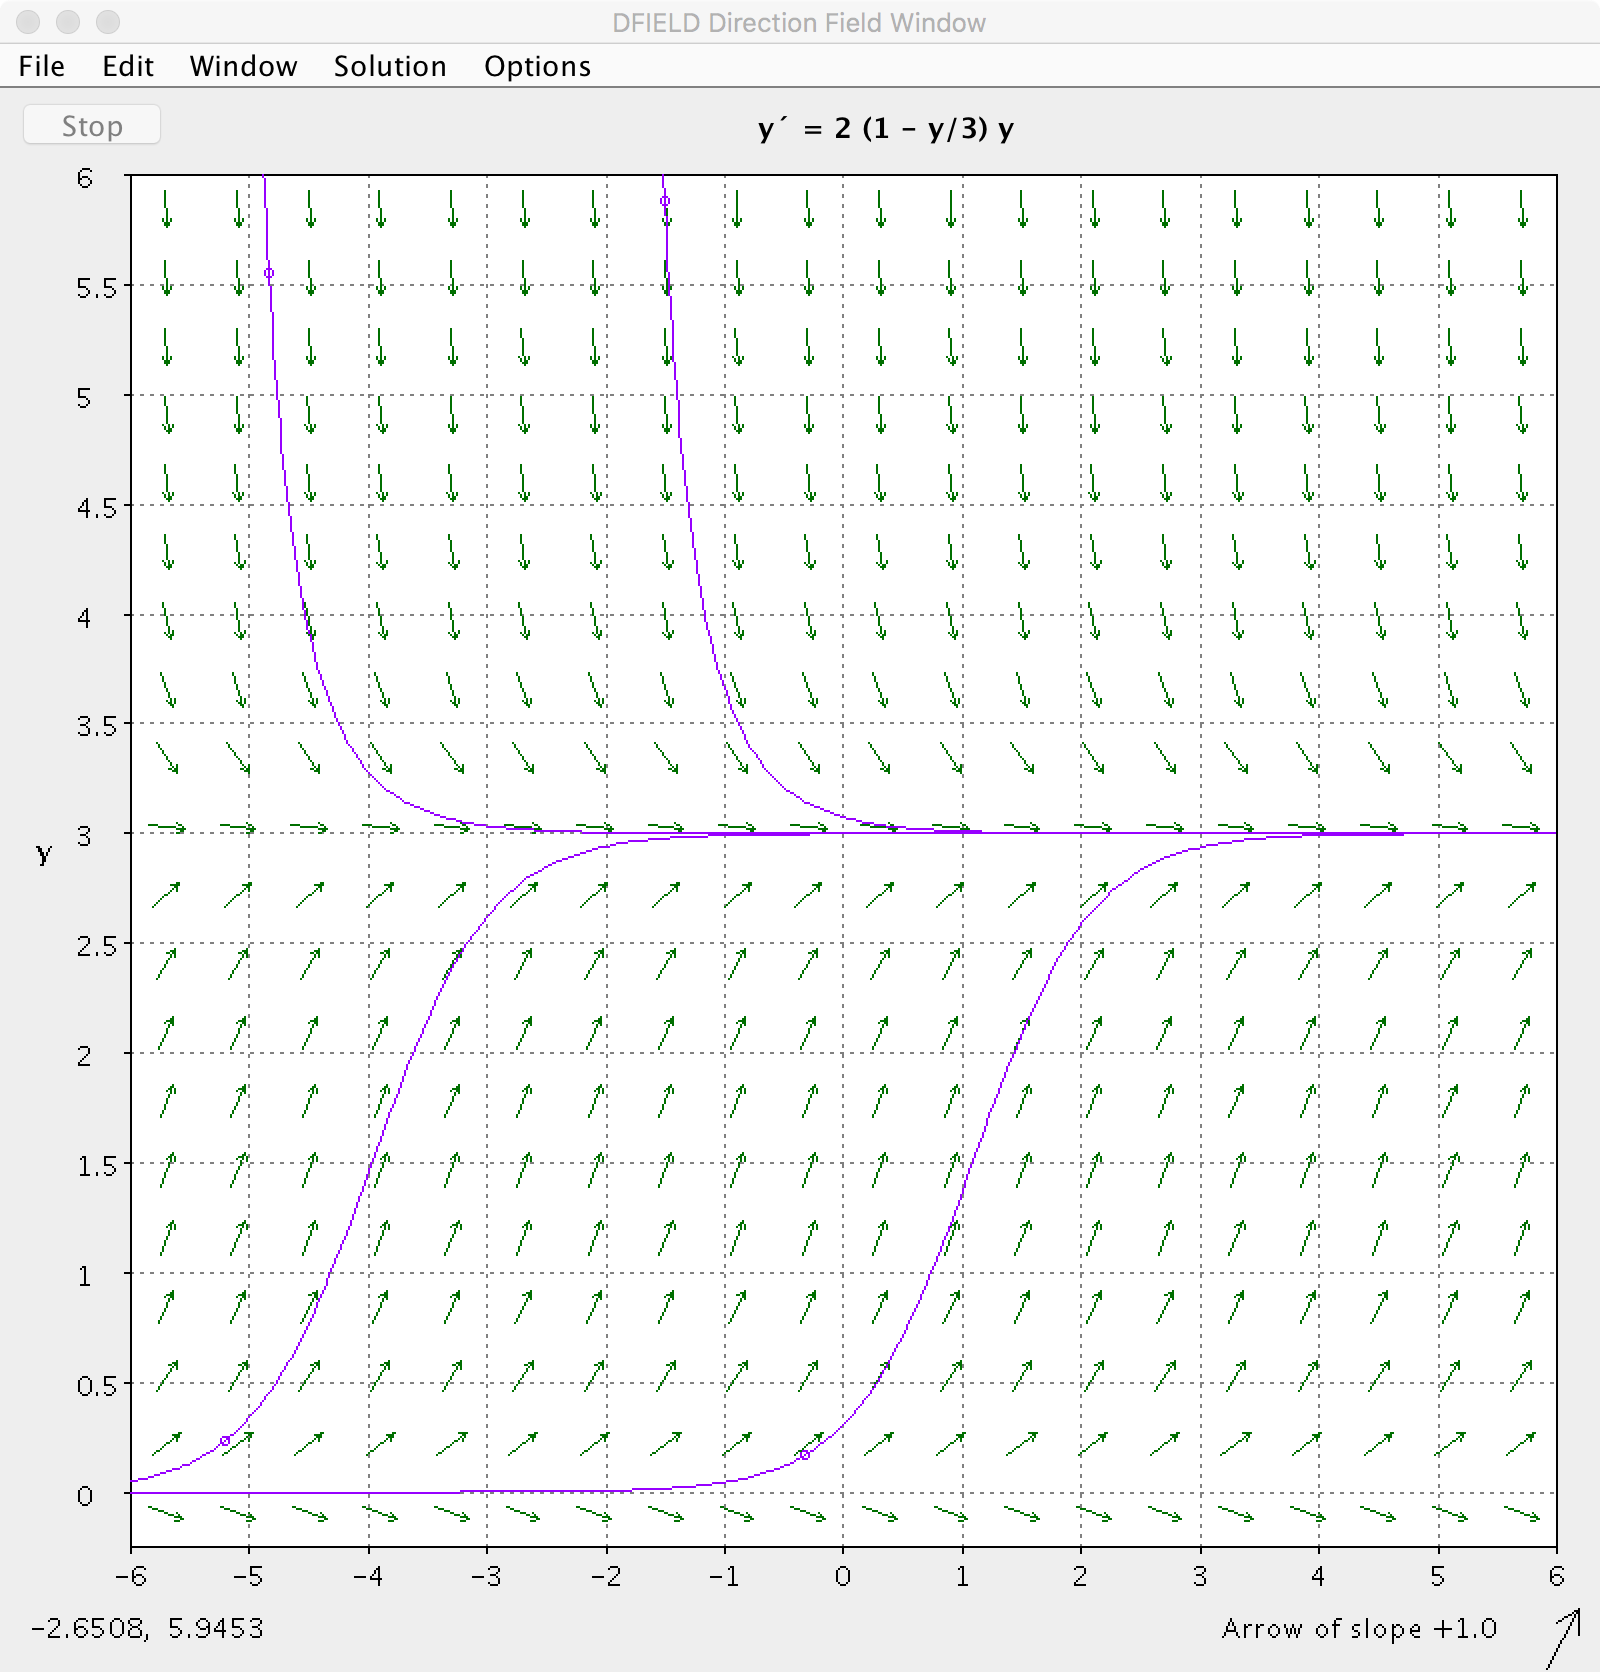
\includegraphics[scale=0.3175]{AutonomousSlope}
		
		\capt{There's software like \texttt{DFIELD} which lets us graph solutions of ODEs without solving them. The goal of this section is to get equally-nice pictures sans slope field!}
	\end{center}
	
	\subsubsection*{Intermediate Goal which will Deliver Us to the Main, Big-Picture Goal}
	In order to get to the $xy$-plane/integral curves we want, we're first going to correctly sketch and label the \textit{phase line} (defined below) corresponding to the given autonomous ODE. 
	
	As shown in class, one of the main tools we're going to use to get \textit{there} is a ``$y$-versus-$f(y)$ graph'' that we're \textit{also} going to construct!

%====================================================================

	\subsection*{How do I know what steps to do when in this nonsense process?!}
	Good question!
	
	While it's not entirely possible to write down a precise recipe for what works for \textit{every} single problem, here's a list that attempts to summarize things somewhat logically (and in-order!).
	\begin{itemize}
		\item Find the \textit{equilibrium solutions} of the ODE. By definition, these will be solutions of the form $y=\const$.
			\begin{itemize}
				\item On the \textbf{``$y$-versus-$f(y)$ graph''}, these will be points/circles \ul{at the values $const$}, \ul{on the $y$-axis}.
				\item On the \textbf{phase line}, these will be points/circles \ul{at the values $\const$}.
				\item On the \textbf{final $xy$-plane graph}, these will be horizontal lines \ul{of the form $y=\const$}.
			\end{itemize}
		\item Find the \textit{local extrema} of the ODE and use these to graph the curve $f(y)$ on the ``$y$-versus-$f(y)$ graph.'' By definition, these will be points where $f'(y)=0$ (see the second part of the below \fbox{boxed} \textbf{note}).
		\begin{itemize}
			\item On the \textbf{``$y$-versus-$f(y)$ graph''}, these will be points/circles \ul{at the local maxes and local mins}.
			\item On the \textbf{phase line}, these will be vertical tick marks \ul{at the values $y$ for which $f'(y)=0$}.
			\item On the \textbf{final $xy$-plane graph}, these will be \ul{$y$-values} marking where the solution curves \ul{change concavity}.
		\end{itemize}
		\item Find where $y$ (as a function of $x$) is \textit{increasing} and \textit{decreasing}.
			\begin{itemize}
				\item On the \textbf{``$y$-versus-$f(y)$ graph''}, these will be regions where the graph of $f(y)$ is \ul{positive} (for increasing) and \ul{negative} (for decreasing).
				\item On the \textbf{phase line}, these will be arrows \ul{pointing right} (for increasing) and \ul{pointing left} (for decreasing).
				\item On the \textbf{final $xy$-plane graph}, these will be \ul{$y$-values} marking where the solution curves are \ul{increasing} and \ul{decreasing}.
			\end{itemize}
		\item Find where $y$ (as a function of $x$) is \textit{concave up} and \textit{concave down}.
		\begin{itemize}
			\item On the \textbf{``$y$-versus-$f(y)$ graph''}, these will be regions where \ul{$f(y)$ and $f'(y)$ have the same signs} (for concave up) and where \ul{$f(y)$ and $f'(y)$ have the opposite signs} (for concave down).
			\item \textbf{You don't put these on the phase line!}
			\item On the \textbf{final $xy$-plane graph}, these will be \ul{$y$-values} marking where the solution curves are \ul{concave up} and \ul{concave down}.
		\end{itemize}
		\item Find the \ul{remaining points} where $y$ (as a function of $x$) has \textit{inflection points}. 
		
		\textbf{Note:} You already found some of these when you found the local extrema of the ODE!
		\begin{itemize}
			\item On the \textbf{``$y$-versus-$f(y)$ graph''}, these will be some (\textbf{but not all!}) of the points where $f(y)$ \ul{has a local max/min} or \ul{crosses the $y$-axis}.
			\item \textbf{If you put these on the phase line} (and you don't have to), they can appear as vertical tick marks.
			\item On the \textbf{final $xy$-plane graph}, these will be \ul{$y$-values} marking where the solution curves \ul{change concavity}.
		\end{itemize}
	\end{itemize}

%====================================================================

	\subsection*{Definitions and Necessary Concepts}
	\begin{defn}
		An ODE is \ul{\textit{autonomous}} if it has the form $\dydx=f(y)$ for some function $f$ (in which $x$ \ul{does not} appear!).
		\begin{adjustwidth}{0.375in}{0.375in}
			\vspace{-6mm}
			\begin{ex}
				$\dydx=y$, $\dydx=2y$, \textellipsis, $\dydx=ny$ ($n=\const$).
			\end{ex}
			\begin{ex}
				$\dydx=y^2$, $\dydx=y^3$, \textellipsis, $\dydx=y^n$ ($n=\const$).
			\end{ex}
			\begin{ex}
				$\dydx=e^y\sin{y}\cos(\cos(\tan{y}))+y\sin{e^{-y^2}}-y^{y^{y^y}}$
			\end{ex}
		\end{adjustwidth}
	\end{defn}

	\notebox{Note:}
	{\vspace{-7.5mm}
		\begin{enumerate}
			\item As shown in class, every autonomous ODE is separable (but not vice versa!); this means that we \textit{can} (and sometimes \textit{will}) solve these ODEs explicitly!
			\item Because $\textstyle dy/dx=f(y)$ and because $y=y(x)$ is a function of $x$, questions requiring the \textit{second} derivative $\textstyle d^2y/dx^2$ of $y$ need the chain rule:
			$$\ddyddx=\frac{d}{dx}\dydx=\frac{d}{dx}f(y(x))=f'(y(x))\,y'(x)=f'(y)f(y).$$
			This verifies the above claim: In order to be concave up (concave down), we need that $\textstyle d^2y/dx^2$ is positive (negative), and $f'(y)f(y)$ is positive (negative) if and only if $f(y)$ and $f'(y)$ have the same (opposite) signs!
		\end{enumerate}
	}

	\begin{defn}
		The \ul{\textit{phase line}} corresponding to an autonomous ODE is a copy of the $y$-axis with information about the equilibrium solutions \textit{and} the increasing/decreasing behavior of $y$ encoded as above.
		\begin{adjustwidth}{0.375in}{0.375in}
			\vspace{-6mm}
			\begin{ex}
				Let $r>0$ and $K>0$ be constants. As we saw in class, 
				$$\dydx=r\left(1-\frac{y}{K}\right)y$$ 
				is an autonomous ODE representing logistic growth, and its corresponding phase line is:
				\vspace{6mm}
				\begin{center}
					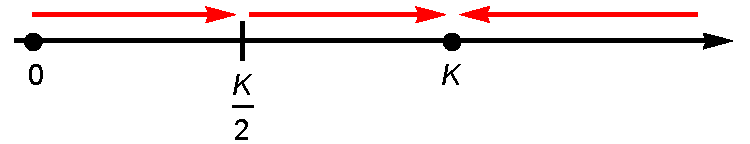
\includegraphics[scale=0.75]{AutonomousPhaseLine1}
				\end{center}
				\vspace{3mm}
				Mathematically, this tells us that the equilibrium solutions for that ODE are $y=0$ and $y=K$, that there is an inflection point at $y=K/2$, and that the solutions must be \textit{increasing} for $y$ in $(0,K)$ and \textit{decreasing} for $y$ in $(K,\infty)$.
				
				\notebox{Note:}
				{We got the data for this phase line by looking at the features of the ``$y$-versus-$f(y)$ graph'' for the ODE. The qualitative analysis used on that graph doesn't tell us \textit{all} the important features possessed by our solutions, however: For instance, we \textit{also} have an inflection point at $y=K$! This point would likely go unnoticed unless you also use other methods of analysis (e.g. studying the derivatives of $f(y)$).}
			\end{ex}
		\end{adjustwidth}
	\end{defn}

	For the sake of convenience, we sometimes add more to the phase line than the bare minimum needed to describe the data mentioned so far. In the example from class, 
	$$\dydx=\underbrace{r\left(1-\frac{y}{K}\right)y}_{f(y)}$$ 
	and in addition to the intervals where $f(y)>0$ and $f(y)<0$ (shown with red arrows above), we can \textit{also} add in information about where $f'(y)>0$ and $f'(y)<0$:
	\begin{center}
		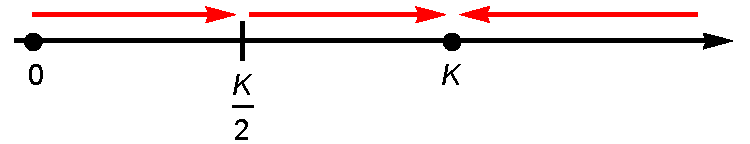
\includegraphics[align=c,scale=0.675]{AutonomousPhaseLine1}
		\hspace{9mm}
		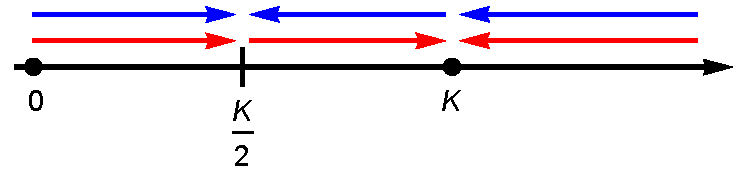
\includegraphics[align=c,scale=0.675]{AutonomousPhaseLine2}
		\vspace{1.5mm}
		\capt{On the left is the ``standard phase line'' discussed above; a modified version of this phase line is on the right. The blue arrows show where $f'(y)>0$ and $f'(y)<0$ with rightward- and leftward-facing arrows, respectively. This modified version will be used throughout.}
	\end{center}
	\vspace{3mm}
	
	And now, one last (pair of) definition(s):
	
	\begin{defn}
		An equilibrium solution $y=\const$ to an ODE is \ul{\textit{asymptotically stable}} if all solutions on both sides of the line $y=\const$ (in the $xy$-plane) limit/converge to $\const$ as $x\to\infty$.
		
		An equilibrium solution $y=\const$ to an ODE is \ul{\textit{asymptotically unstable}} if \ul{no} solutions on either side of the line $y=\const$ (in the $xy$-plane) limit/converge to $\const$ as $x\to\infty$. In particular, the equilibrium solution $y=\const$ is asymptotically unstable if and only if the only solution to the ODE which ``always stays close'' to $y=\const$ as $x\to\infty$ is $y=\const$ itself.
	\end{defn}
	
	There are other related notions, too, like ``semistable solutions,'' etc.; before saying too many more words, however, I think it's time to shift to some examples!
	
%====================================================================

	\subsection*{Example 1}
	In this example, we're going to consider the autonomous ODE
	\begin{equation}
		\label{eq:ex1}
		\dydx = \underbrace{-r\left(1-\frac{y}{T}\right) y}_{f(y)}.
	\end{equation}
	Here, $r>0$ and $T>0$ are positive constants. To graph the solutions of \eqref{eq:ex1}, we're going to break the process into steps as described above.

	\subsubsection*{Equilibrium solutions:}\par
	Recall that an \textit{equilibrium solution} is a solution of the form $y=\const$ so that $\dydx=0$. In this case,
	\begin{equation}\label{eq:Eq1}\dydx=0\iff-r=0\text{\hspace{3mm}\ul{or}\hspace{3mm}}1-\frac{y}{T}=0\text{\hspace{3mm}\ul{or}\hspace{3mm}}y=0;\end{equation}
	because $r\neq 0$ is assumed, the equilibrium solutions are $y=T$ and $y=0$. We plot those on the ``$y$-versus-$f(y)$ graph'' and on the phase line.
	\begin{center}
		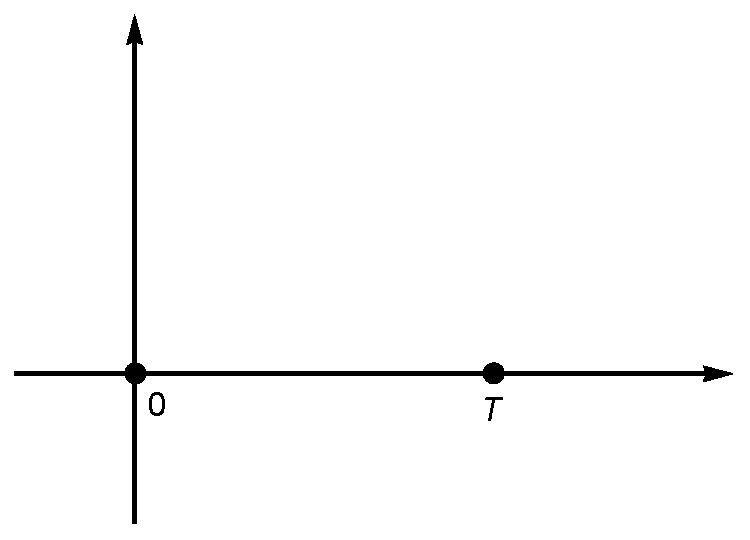
\includegraphics[align=c,scale=0.675]{Ex1_yf(y)_1}
		\hspace{9mm}
		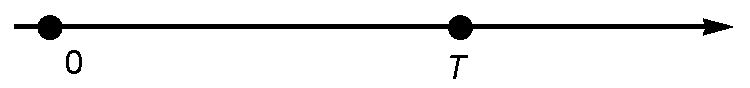
\includegraphics[align=c,scale=0.675]{Ex1_Phase_1}
		\vspace{1.5mm}
		\capt{On the left, the ``$y$-versus-$f(y)$ graph''; the phase line is on the right. We'll continue to post updated versions as we go.}
	\end{center}

	\subsubsection*{Sketch the ``$y$-versus-$f(y)$'' curve:}\par
	By manipulating equation \eqref{eq:ex1}, we see that
	$$f(y)=-ry+\frac{r}{T}y^2$$
	has a graph which is an upward-facing parabola with respect to $y$. Before proceeding, we want to sketch what that looks like on the ``$y$-versus-$f(y)$'' graph.
	
	In order to do this step, we need to find the vertex (or \textit{local min}) of the parabola. To do this, we \ul{can} use the formula
	$$\text{vertex}=\left(\frac{-b}{2a},f\left(\frac{-b}{2a}\right)\right),$$
	but for later examples, what we'll see is that finding the \textit{critical points} for $f(y)$ (i.e., where $f'(y)=0$) will work in the most general cases.
	
	Using the second part of the above \fbox{boxed} \textbf{note}, it follows that
	\begin{equation}
		\label{eq:CritPt1}
		\ddyddx=f(y)f'(y)=\underbrace{\left(-r\left(1-\frac{y}{T}\right) y\right)}_{f(y)}\,\underbrace{\left(-r+\frac{2r}{T}y\right)}_{f'(y)},
	\end{equation}
	and the critical points for $f$ will be where $f(y)=0$ and $f'(y)=0$. In particular, $f(y)=0$ yields the critical points already found in \eqref{eq:Eq1}; $f'(y)=0$ yields one new critical point, namely
	$$y=\frac{T}{2}.$$
	Plugging into $f$, we see that the vertex of the parabola is
	\begin{equation}
		\label{eq:Ex1Vertex}
		\left(\frac{T}{2},f\left(\frac{T}{2}\right)\right)=\left(\frac{T}{2},\frac{-rT}{4}\right),
	\end{equation}
	and now, we represent the data in \eqref{eq:Ex1Vertex} on both the ``$y$-versus-$f(y)$ graph'' and the phase line:
	\begin{center}
		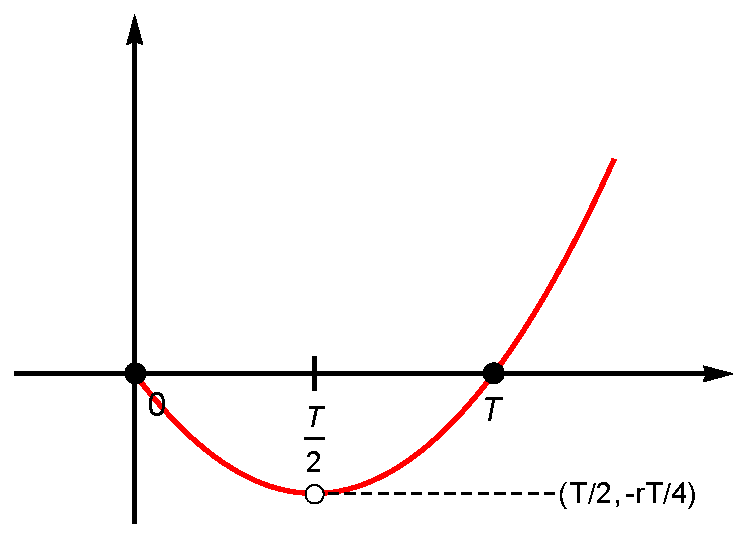
\includegraphics[align=c,scale=0.675]{Ex1_yf(y)_2}
		\hspace{9mm}
		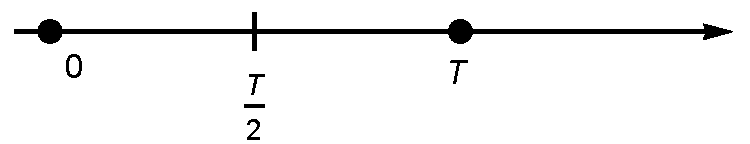
\includegraphics[align=c,scale=0.675]{Ex1_Phase_2}
		\vspace{1.5mm}
		\capt{On the left is the ``$y$-versus-$f(y)$ graph'' featuring the newly-added vertex; the corresponding phase line is on the right.}
	\end{center}

	\subsubsection*{Determine where $y$ is increasing and decreasing:}\par
	By definition, 
	\begin{itemize}
		\item $y$ is increasing as a function of $x$ when the ``$y$-versus-$f(y)$'' curve is \ul{above} the $y$-axis; and
		\item $y$ is decreasing as a function of $x$ when the ``$y$-versus-$f(y)$'' curve is \ul{below} the $y$-axis.
	\end{itemize}

	Based on the above figure, the ``$y$-versus-$f(y)$'' curve is below the $y$-axis for $0<y<T$ and above the $y$-axis for $y>T$. Thus, 
	$$y\text{ is \ul{increasing} on }(T,\infty)\text{ and }y\text{ is \ul{decreasing} on }(0,T).$$
	
	Now, we encode that data on the phase line by putting a \textbf{rightward} arrow on intervals where $y$ is increasing and a \textbf{leftward} arrow where $y$ is decreasing.
	\vspace{1.5mm}
	\begin{center}
		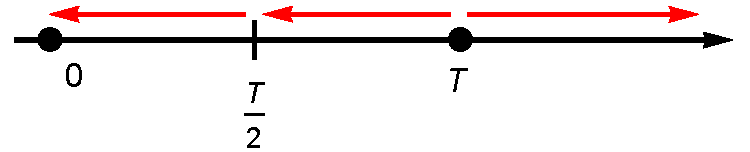
\includegraphics[align=c,scale=0.75]{Ex1_Phase_3}
		\vspace{1.5mm}
		\capt{Encoding increasing/decreasing information on the phase line.}
	\end{center}

	\subsubsection*{Determine where $y$ is concave up and concave down:}\par
	In particular, we want to figure out where $\ddyddx>0$ and $\ddyddx<0$, and to do so, we refer back to equation \eqref{eq:CritPt1} and notice that
	$$\ddyddx=f(y)f'(y)>0\iff f(y)\text{ and }f'(y)\text{ have the same sign};$$
	similarly, 
	$$\ddyddx<0$$ whenever $f(y)$ and $f'(y)$ have opposite signs.
	
	By determining where $y$ is increasing and decreasing, we've figured out where $f(y)>0$ and $f(y)<0$, respectively. Therefore, we only need to examine the sign of
	$$f'(y)=-r+\frac{2r}{T}y,$$
	and we see\footnote{You can also just look at where the graph of $f(y)$ is increasing/decreasing. These notions are equivalent.} that $f'(y)>0\iff -r+\frac{2r}{T}y>0\iff y>\frac{T}{2}$. We combine this data with the phase line as follows\footnote{This isn't something you \ul{have} to do: I do it here for clearer exposition.}:
	\begin{center}
		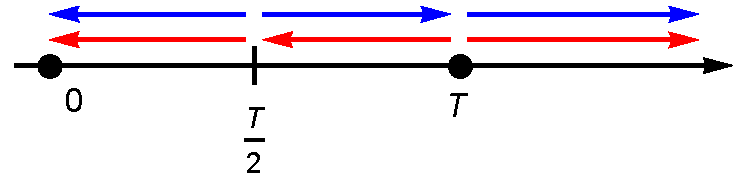
\includegraphics[align=c,scale=0.75]{Ex1_Phase_4}
		\vspace{1.5mm}
		\capt{Encoding on the phase line where $f(y)>0$, $f(y)<0$ \textbf{and} where $f'(y)>0$, $f'(y)<0$. As before, the red rightward and leftward arrows indicate where $f(y)>0$ and $f(y)<0$, respectively (i.e. where $y$ is increasing and decreasing, respectively). A new addition is the blue rightward and leftward arrows, indicating intervals where $f'(y)>0$ and $f'(y)<0$, respectively.}
	\end{center}

	Based on the dialogue above, $y$ is concave \ul{up} on intervals where the red and blue arrows are pointing in the \ul{same} direction and concave \ul{down} when the red and blue arrows are pointing in \ul{opposite} directions. We indicate this as follows:
	\begin{center}
		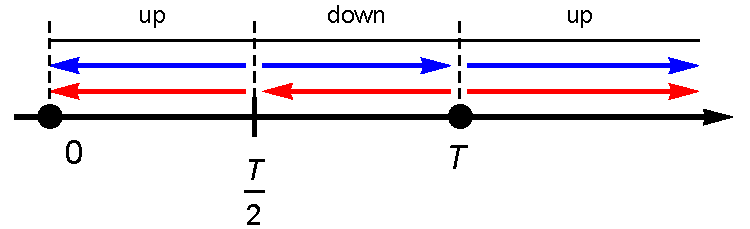
\includegraphics[align=c,scale=0.875]{Ex1_Phase_5}
		\vspace{1.5mm}
		\capt{Encoding concavity on the phase line. As stated, $y$ is concave \ul{up} when $f$ and $f'$ have the same sign (i.e. when the red and blue arrows are pointing in the same direction); it's concave \ul{down} otherwise.}
	\end{center}
	As \textbf{intervals}, we have:
	$$y\text{ is concave \ul{up} on }\left(0,\frac{T}{2}\right)\cup(T,\infty)\text{ and }y\text{ is concave \ul{down} on }\left(\frac{T}{2},T\right).$$
	
	\subsubsection*{Determine the inflection points of $y$:}\par
	After filling in the last phase line, this data is given for free:
	$$y\text{ has inflection points when }y=\frac{T}{2}\text{ and when}y=T.$$
	
	\subsubsection*{Turning phase lines into drawn graphs}
	First, we rotate the phase line so that it's vertical and we place it next to an empty $xy$-plane:
	\vspace{-6mm}
	\begin{center}
		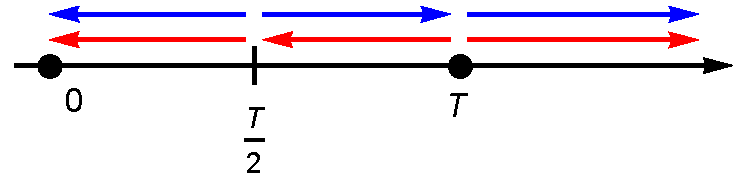
\includegraphics[align=c,scale=0.5]{Ex1_Phase_4}
		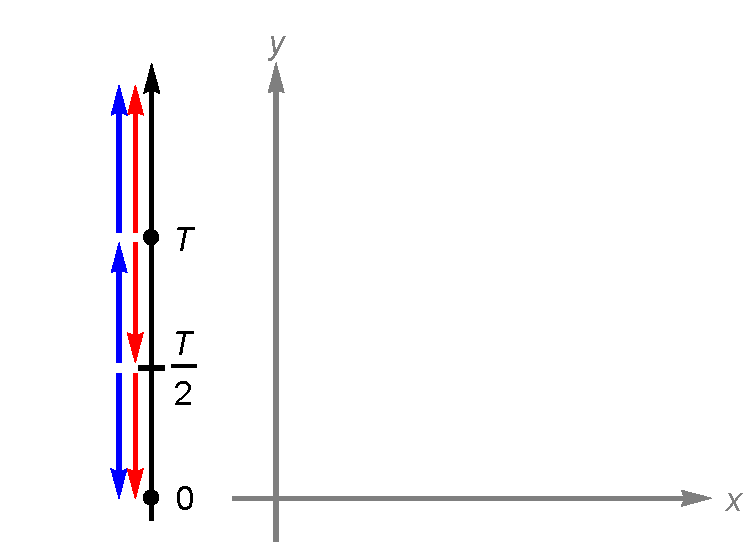
\includegraphics[align=c,scale=0.875]{Ex1_xy_1}
		\vspace{1.5mm}
		\capt{The phase line (on the left) is flipped and put next to an empty $xy$-plane.}
	\end{center}
	Next, we plot the equilibrium solutions $y=0$ and $y=T$ on the $xy$-plane; I'll also add in a dotted line corresponding to the inflection point $y=T/2$, though this is optional.
	\begin{center}
		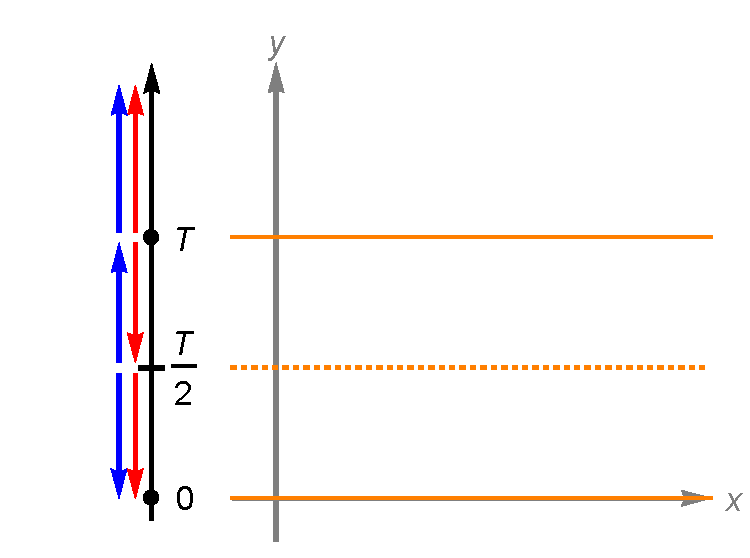
\includegraphics[align=c,scale=0.875]{Ex1_xy_2}
		\vspace{1.5mm}
		\capt{The equilibrium solutions are added (in orange).}
	\end{center}
	The data we have on solutions $y$ is as follows:
	\begin{itemize}
		\item $y$ should be decreasing and concave up on $(0,T/2)$;
		\item $y$ should be decreasing and concave down on $(T/2,T)$; and
		\item $y$ should be increasing and concave up on $(T,\infty)$.
	\end{itemize}
	That means that $y$ should look like exponential growth on the interval $(T,\infty)$ and should look like the flipped version of the ``logistic growth elongated S-shape'' on $(0,T)$:
	\vspace{-6mm}
	\begin{center}
		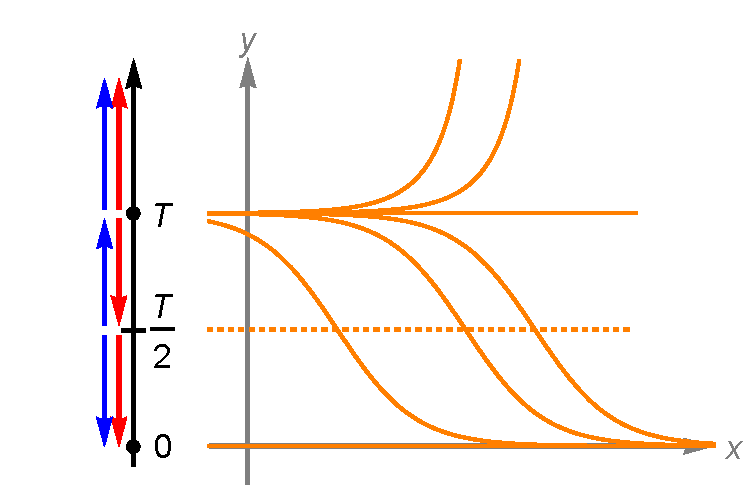
\includegraphics[align=c,scale=1]{Ex1_xy_3}
		\vspace{1.5mm}
		\capt{A sketch of various solutions (in orange) to the {\normalfont{ODE}} $\dydx = -r\left(1-\frac{y}{T}\right) y$.}
	\end{center}

	\subsubsection*{Conclusion}
	Based on the above graphical information, we can say that 
	\begin{itemize}
		\item $y=T$ is \textbf{asymptotically unstable}, as the only solution that ``stays near $y=T$ for large $x$'' is $y=T$ itself;
		\item $y=0$ is \textbf{asymptotically stable}. We can see this by extending the model to allow for solutions $y<0$ (see graph on next page), in which case we see that all solutions in the intervals $0<y<T$ \ul{and} $y<0$ tend towards $0$ as $x\to\infty$.
	\end{itemize}	

	\newpage
	
	\vspace*{\fill}
	\begin{center}
		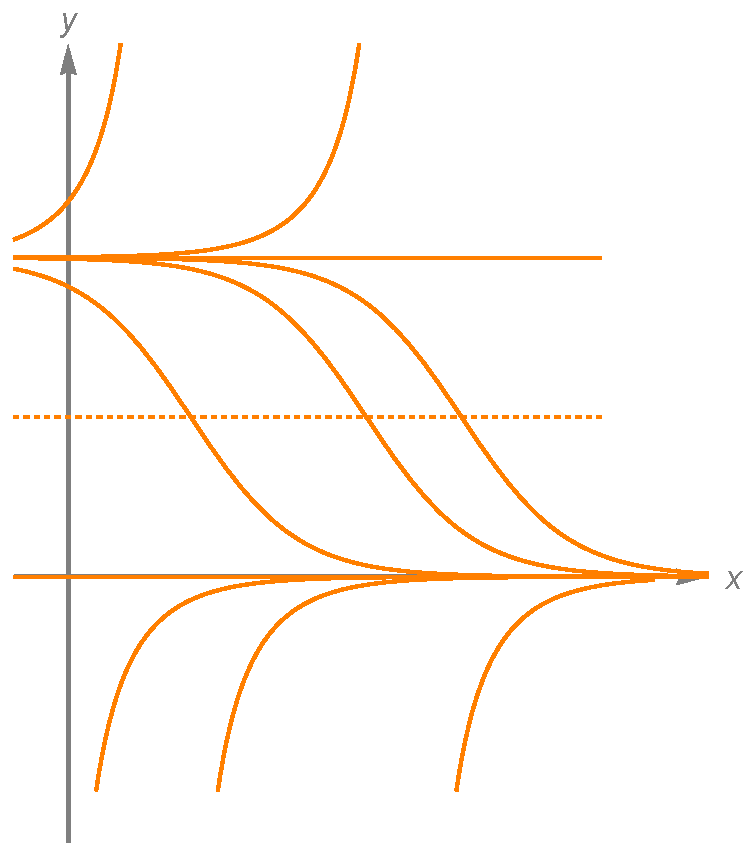
\includegraphics[scale=1]{Ex1_xy_4}
		\vspace{1.5mm}
		\capt{A sketch of various solutions (in orange) to the {\normalfont{ODE}} $\textstyle \dydx = -r\left(1-\frac{y}{T}\right) y$ where here, we allow $y<0$ to occur. Notice that all solutions in the intervals $0<y<T$ \ul{and} $y<0$ tend towards $0$ as $x\to\infty$.}
	\end{center}
	\vspace*{\fill}
	
	\newpage
	
%====================================================================

	\subsection*{Example 2}
	In this example, we're going to consider the somewhat more difficult autonomous ODE
	\begin{equation}
		\label{eq:ex2}
		\dydx = \underbrace{-r\left(1-\frac{y}{T}\right)\left(1-\frac{y}{K}\right) y}_{f(y)}.
	\end{equation}
	Here, we assume that $r$, $T$, and $K$ are positive constants; \ul{this time, we further assume that $0<T<K$}. As above, we're going to graph the solutions of \eqref{eq:ex2} by breaking the process into the appropriate steps.
	
	\subsubsection*{Equilibrium solutions:}\par
	We again consider the equation $\dydx=0$, and here,
	$$\dydx=0\iff-r=0\text{\hspace{3mm}\ul{or}\hspace{3mm}}1-\frac{y}{T}=0\text{\hspace{3mm}\ul{or}\hspace{3mm}}1-\frac{y}{K}=0\text{\hspace{3mm}\ul{or}\hspace{3mm}}y=0.$$
	Again, $r\neq 0$, so this time, there are \textit{three} equilibrium solutions: $y=T$, $y=K$, and $y=0$. As above, we plot those on the ``$y$-versus-$f(y)$ graph'' and on the phase line.
	\begin{center}
		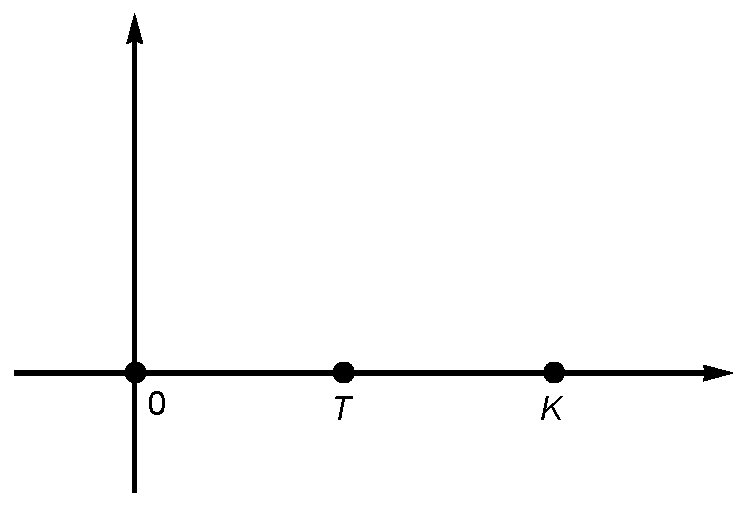
\includegraphics[align=c,scale=0.675]{Ex2_yf(y)_1}
		\hspace{9mm}
		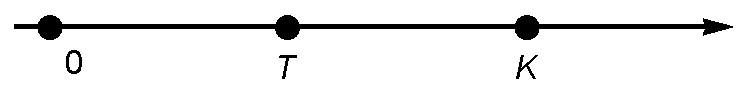
\includegraphics[align=c,scale=0.675]{Ex2_Phase_1}
		\vspace{1.5mm}
		\capt{On the left, the ``$y$-versus-$f(y)$ graph''; the phase line is on the right. Note that we \textbf{assumed} that $0<T<K$; otherwise, we wouldn't know whether $T$ or $K$ was leftmost.}
	\end{center}

	\subsubsection*{Sketch the ``$y$-versus-$f(y)$'' curve:}\par
	From equation \eqref{eq:ex2},
	$$f(y)=-\frac{r y^3}{K T}+\frac{r y^2}{K}+\frac{r y^2}{T}-r y,$$
	and on the ``$y$-versus-$f(y)$ graph,'' this curve is a cubic whose graph approaches $+\infty$ as $y\to-\infty$ and $-\infty$ as $y\to+\infty$; in particular, it starts at the ``top left'' and is directed towards the ``bottom right.'' We want to fill in the distinguishing features of the graph before proceeding.
	
	As before, we'll use the second part of the above \fbox{boxed} \textbf{note}:
	\begin{equation}
	\label{eq:CritPt2}
	\ddyddx=f(y)f'(y)=\underbrace{\left(-r\left(1-\frac{y}{T}\right)\left(1-\frac{y}{K}\right) y\right)}_{f(y)}\,\underbrace{\left(-\frac{3 r y^2}{K T}+\frac{2 r y}{K}+\frac{2 r y}{T}-r\right)}_{f'(y)}.
	\end{equation}
	Once again, we identify the new critical points to be the values $y$ for which $f'(y)=0$, namely those $y$ for which
	\begin{equation}
		\label{eq:Ex2Quad}
		-\frac{3 r y^2}{K T}+\frac{2 r y}{K}+\frac{2 r y}{T}-r=0;
	\end{equation}
	solving this equation requires the quadratic formula, but doing so yields two solutions $y_1$ and $y_2$ of the form
	$$y_1=\frac{1}{3} \left(K+T-\sqrt{K^2-K T+T^2}\right)\hspace{3mm}\text{and}\hspace{3mm}y_2=\frac{1}{3} \left(K+T+\sqrt{K^2-K T+T^2}\right).$$
	We won't worry about plugging these into $f$ to find $f(y_1)$ or $f(y_2)$; instead, we note simply that $f(y_1)<0$ and $f(y_2)>0$. This is enough to represent the data on both the ``$y$-versus-$f(y)$ graph'' and the phase line:
	\begin{center}
		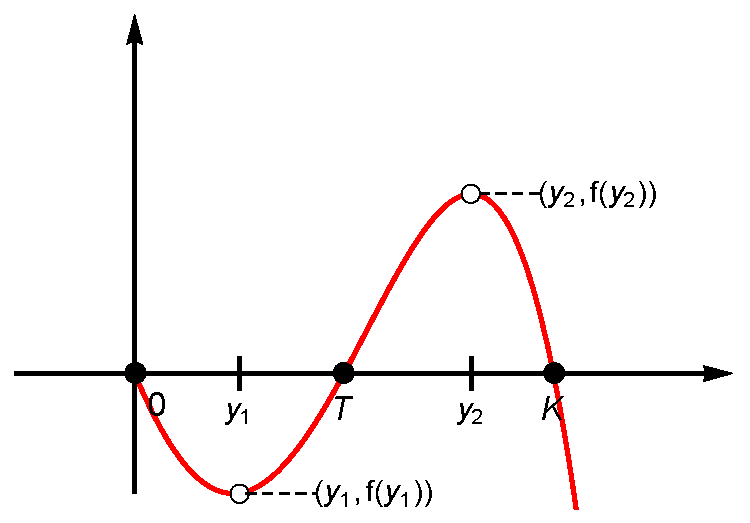
\includegraphics[align=c,scale=0.675]{Ex2_yf(y)_2}
		\hspace{9mm}
		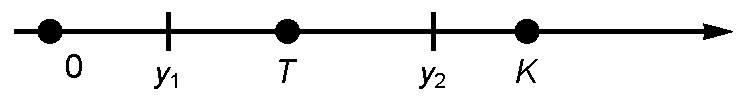
\includegraphics[align=c,scale=0.675]{Ex2_Phase_2}
		\vspace{1.5mm}
		\capt{On the left is the ``$y$-versus-$f(y)$ graph'' featuring the newly-added local extrema; the corresponding phase line is on the right.}
	\end{center}

	\subsubsection*{Determine where $y$ is increasing and decreasing:}\par
	As in the first example, $y$ is increasing (decreasing) as a function of $x$ when the ``$y$-versus-$f(y)$'' curve is \ul{above} (\ul{below}) the $y$-axis.
	
	Based on the above figure, the ``$y$-versus-$f(y)$'' curve is above the $y$-axis for $T<y<K$ and below the $y$-axis elsewhere (for $0<y<T$ and for $y>K$). Thus, $y$ is \textbf{increasing} on the interval $(T,K)$ and is \textbf{decreasing} on the set $(0,T)\cup(K,\infty)$.
	
	This is shown on the following phase line.
	
	\begin{center}
		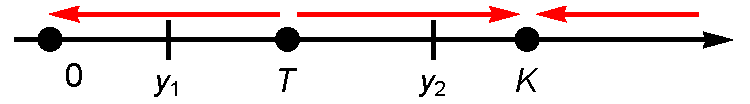
\includegraphics[align=c,scale=0.75]{Ex2_Phase_3}
		\vspace{1.5mm}
		\capt{Encoding increasing/decreasing information on the phase line.}
	\end{center}

	\subsubsection*{Determine where $y$ is concave up and concave down:}\par
	Looking at the ``$y$-versus-$f(y)$'' curve, we see that $f(y)$ is \ul{increasing} on the interval $(y_1,y_2)$ and is \ul{decreasing} on $(0,y_1)\cup(y_2,\infty)$. We can put this on the phase line using blue arrows:
	\begin{center}
		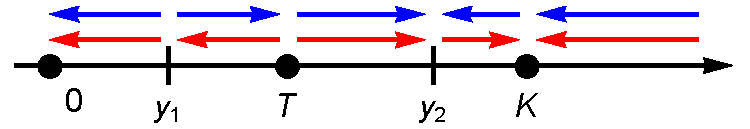
\includegraphics[align=c,scale=0.75]{Ex2_Phase_4}
		\vspace{1.5mm}
		\capt{Encoding on the phase line where $f(y)>0$, $f(y)<0$ \textbf{and} where $f'(y)>0$, $f'(y)<0$ with red and blue arrows, respectively.}
	\end{center}

	\noindent And now, we make the concavity labeling explicit
	\begin{center}
		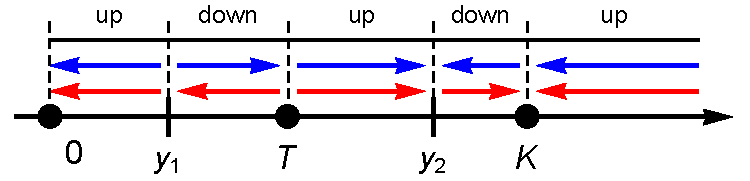
\includegraphics[align=c,scale=0.875]{Ex2_Phase_5}
		\vspace{1.5mm}
		\capt{Encoding concavity on the phase line. As stated, $y$ is concave \ul{up} when $f$ and $f'$ have the same sign (i.e. when the red and blue arrows are pointing in the same direction); it's concave \ul{down} otherwise.}
	\end{center}
	As \textbf{intervals}, we have:
	$$y\text{ is concave \ul{up} on }\left(0,y_1\right)\cup(T,y_2)\cup(K,\infty)\text{ and }y\text{ is concave \ul{down} on }(y_1,T)\cup(y_2,K).$$
	
	\vspace{6mm}
	\subsubsection*{Determine the inflection points of $y$:}\par
	After filling in the last phase line, this data is given for free:
	$$y\text{ has inflection points when }y=y_1, y=T, y=y_2,\text{ and }y=K.$$

	\subsubsection*{Turning phase lines into drawn graphs}
	As above, we rotate the phase line so that it's vertical and we place it next to an empty $xy$-plane:
	\vspace{-1.5mm}
	\begin{center}
		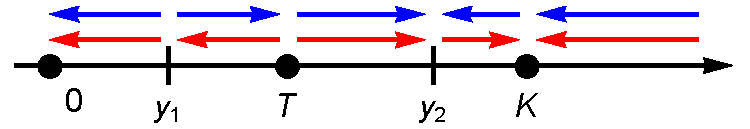
\includegraphics[align=c,scale=0.5]{Ex2_Phase_4}
		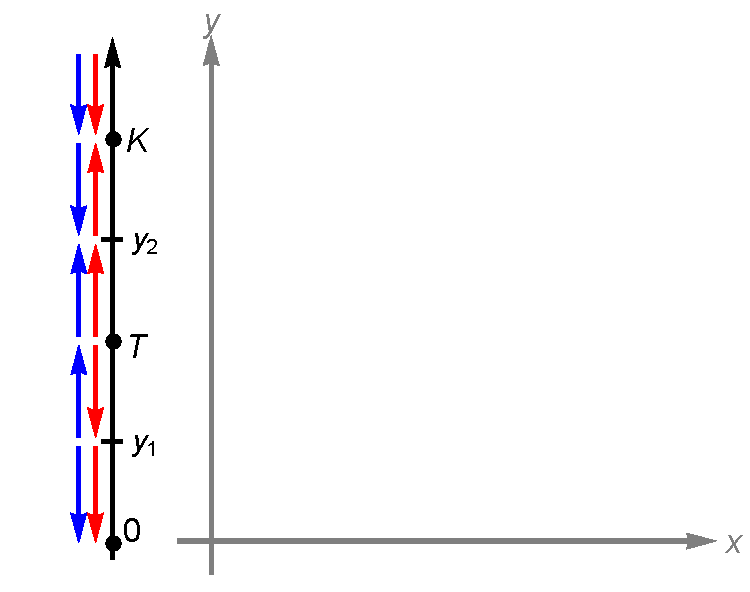
\includegraphics[align=c,scale=0.875]{Ex2_xy_1}
		\vspace{1.5mm}
		\capt{The phase line (on the left) is flipped and put next to an empty $xy$-plane.}
	\end{center}
	Next, we plot the equilibrium solutions $y=0$, $y=T$, and $y=K$ on the $xy$-plane; as above, I've also added a(n optional) dotted line corresponding to the inflection points $y=y_1$ and $y=y_2$.
	\begin{center}
		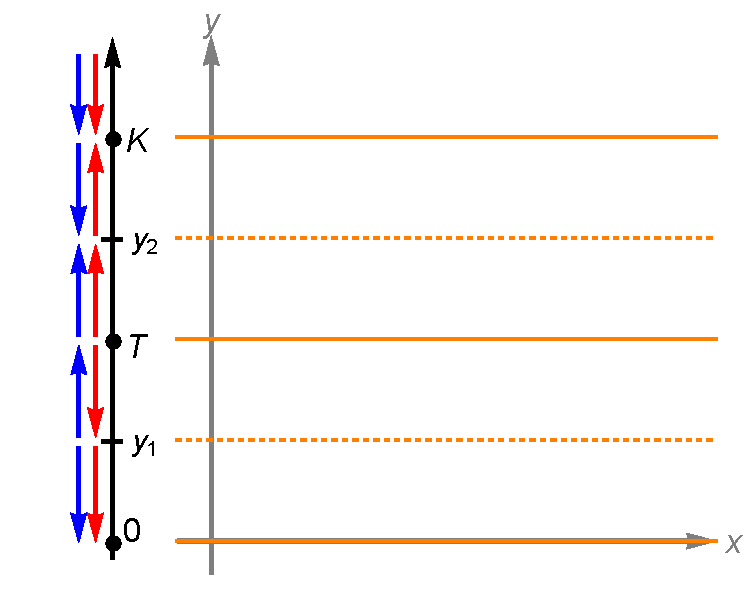
\includegraphics[align=c,scale=0.875]{Ex2_xy_2}
		\vspace{1.5mm}
		\capt{The equilibrium solutions are added (in orange).}
	\end{center}
	The data we have on solutions $y$ is as follows:
	\begin{itemize}
		\item $y$ should be decreasing and concave up on $(0,y_1)$;
		\item $y$ should be increasing and concave down on $(y_1,T)$; 
		\item $y$ should be increasing and concave up on $(T,y_2)$;
		\item $y$ should be decreasing and concave down on $(y_2,K)$; and
		\item $y$ should be decreasing and concave up on $(K,\infty)$;
	\end{itemize}
	That means that $y$ should look like exponential decay on the interval $(K,\infty)$, like the ``logistic growth elongated S-shape'' on $(T,K)$, and like the flipped version of the ``logistic growth elongated S-shape'' on $(0,T)$. 
	
	The graph (on the next page) matches this intuition.

	\subsubsection*{Conclusion}
	As above, we can extend the ODE to allow for solutions $y<0$ (not pictured), and doing so would show that
	\begin{itemize}
		\item $y=K$ is \textbf{asymptotically stable};
		\item $y=T$ is \textbf{asymptotically unstable}; and
		\item $y=0$ is \textbf{asymptotically stable}.
	\end{itemize}	

	\vspace{-6mm}
	\begin{center}
		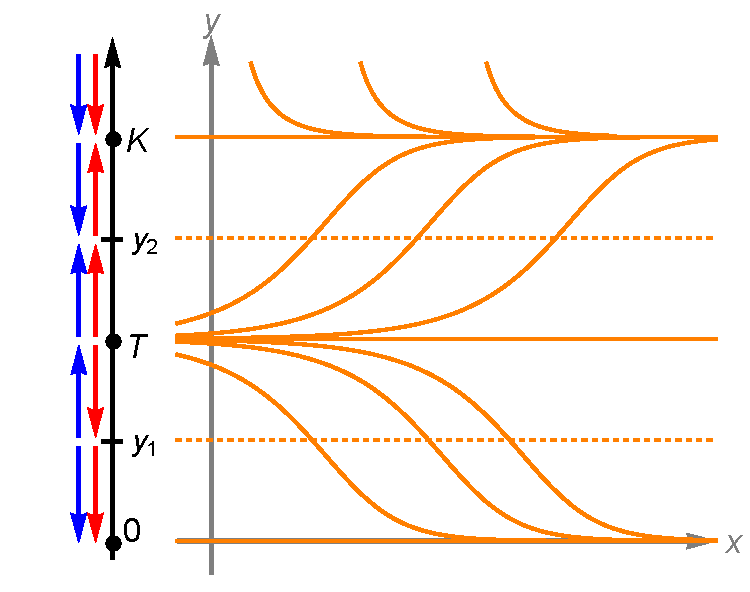
\includegraphics[align=c,scale=1]{Ex2_xy_3}
		\vspace{1.5mm}
		\capt{A sketch of various solutions (in orange) to the {\normalfont{ODE}} $\dydx = -r\left(1-\frac{y}{T}\right)\left(1-\frac{y}{K}\right) y$.}
	\end{center}

	% Mention intial value stuff
\end{document}